\chapter{Analýza súčasného stavu}


%z knihy od michal gregor - umela inteligencia
%na strane 11 a 12 cituje v clanku ref 13

%11 strana knihy o umelej inteligenciie z od gregora
%doslovné citovanie
Fuzzy prístupy možno považovať za odpoveď na požiadavku spracovania neurčitosti, resp. nepresnosti. Táto požiadavka je veľmi rozšírená - v určitej forme sa vyskytuje prakticky v každom reálnom systéme aplikujúcom metódy umelej inteligencie - predovšetkým sa však objavuje tam, kde systémy nejakým spôsobom interferujú s človekom alebo využívajú ľudské znalosti \cite{gregorUI} .

V súvislosti s neurčitosťou sa rozlišujú tri základné pojmy:   %tuto cituje [13] (Niklesa) 
%todo prestylizovat toto!!!
\begin{itemize}
	\item \textbf{Neurčitosť} - vyplýva z nedostatočnej znalosti faktorov alebo udalosti. O neurčitosti sa hovorí, že je aleatórna, ak pramení z vnútorných vlastností nejakého náhodného javu - t.j. ju principiálne nemožno odstrániť. Ak neurčitosť vyplýva z neznalosti, tak je epistemická. 
	\item \textbf{Nepresnosť} - O nepresnosti hovoríme, ak je znalosť faktov a udalosti taká kompletná ako len môže byť, ale spôsob ich vyjadrenia nie je presný alebo jednoznačný. 
	\item \textbf{Nekonzistentnosť} - O nekonzistentnosti sa hovorí, ak si znalosti, resp. známe fakty navzájom odporujú\cite{ gregorUI,gregorRef13}.
\end{itemize} 

%12 strana knihy umela inteligencia
Ľudské znalosti vo väčšine prípadov zahŕňajú neurčitosti, nepresnosť, niekedy môžu byť aj nekonzistentné. 
Fuzzy prístupy umožňujú určitým spôsobom formalizovať a ďalej spracúvať vágne poznatky. Vágnosť možno považovať za typ nepresnosti. 
%tuto on cituje 13
Takýto typ znalostí je ťažké a často aj nemožné vhodne formalizovať konvenčnými metódami. Fuzzy prístupy predstavujú jednu z možných ciest ako k nim pristupovať, a použiť na formalizáciu neurčitosti \cite{gregorUI, gregorRef13}.

Teória fuzzy množín je zovšeobecnením klasickej teórie množín - fuzzy množiny sú vágne v tom či prvok patrí alebo nepatrí do množiny.  Na fuzzy množinách možno vykonávať určité operácie čiastočne analogické s tými, ktoré sú v klasickej teórie množín. Fuzzy logika predstavuje prístup, ktorý zovšeobecňuje konvenčnú logiku a produkčné pravidlá zavedením tzv. lingvistických premenných a lingvistických pravidiel. Fuzzy logika umožňuje formulovať vágne pravidlá. Fuzzy aritmetika rozširuje princípy klasickej aritmetiky na vágne - fuzzy - čísla \cite{gregorUI}. 


% tieto pojmy asi su aj v Zadeh1965, Zadeh1996 , citujem ich doslovne z knihy = Projektovanie systemov.. 

\section{Teória fuzzy množín}
Nech \textit{$ X = \left\lbrace x \right\rbrace$} je množina prvkov \textit{x}. 

\subsection*{Fuzzy množina}
\begin{defn} 
	
	Fuzzy množina \textit{$A \subset X $} je predstavovaná množinou dvojíc $ \left\lbrace \left( x, \mu_A \left( x \right) \right) \right\rbrace  $, kde $ x \in X$ a $ \mu_A : X \longrightarrow \left\langle 0, 1\right\rangle $ je funkcia príslušnosti, ktorá predstavuje subjektívnu mieru príslušnosti elementu \textit{x} k množine \textit{A}. 
	Veličina $\mu_A\left( x\right) $ nadobúda hodnoty od nuly, ktorá označuje absolútnu príslušnosť po hodnotu jedna, ktorá hovorí o absolútnej príslušnosti elementu \textit{x} do fuzzy množiny \textit{A} \cite{levashenkoProj, Zadeh1965}.\end{defn}

%12 strana knihy o projektovani systemov
Ak je fuzzy množina \textit{A} definovaná na konečnej univerzálnej množine 
\\
$X = \left\lbrace x_1, x_2, \ldots , x_i, \ldots, x_n\right\rbrace $, potom je vhodné označiť ju nasledovne
$$
A = \left\lbrace 
\left( x_1, \mu_A\left( x_1\right)  \right) , 
\left( x_2, \mu_A\left( x_2\right)  \right) , ... , 
\left( x_i, \mu_A\left( x_i\right)  \right) , ... , 
\left( x_n, \mu_A\left( x_n\right)  \right) 
\right\rbrace , 
$$ 
kde $\left( x_i, \mu_A\left( x_i\right)  \right)$ - je dvojica tvorená elementov $x_i$ a jeho funkciou príslušnosti, nazývaná singleton \cite{levashenkoProj}. 

%%tieto definicie su na strane 12, a su citovane z knihy, a aj Kaufmann1985, Klir1995, Navara2011




\subsection*{Fuzzy premenná}

\begin{defn}
Fuzzy premenná je definovaná trojicou $\left( \alpha, X, A \right) $, kde 
$\alpha $ - je meno fuzzy premennej, 
 $X=\left\lbrace x \right\rbrace$ - je množina, tvoriaca definičný obor premennej \textit{x}, 
 \textit{A} - je fuzzy podmnožina fuzzy množiny \textit{X}, pre každý prvok ktorej je definovaná funkcia $\mu_A\left( x\right)$, udávajúca stupeň príslušnosti daného elementu \textit{x} do množiny \textit{A}   \cite{levashenkoProj}.\end{defn}


\subsection*{Lingvistická premenná}
Lingvistická, resp. jazyková premenná je zvláštnym typom premennej, ktorá sa od numerických premenných odlišuje tým, že jej hodnoty - tzv. lingvistické hodnoty - nie sú čísla, ale slovné výrazy. Pritom každej lingvistickej hodnote je priradený význam, t. j. určitá fuzzy množina definovaná na spoločnom univerze \cite{gregorUI}.
\begin{defn} 
	Lingvistická premenná je definovaná päticou \textit{$\left(\beta, T, X, G, M \right) $}, kde 
	$\beta$ - je meno lingvistickej premennej; 
	\textit{T} - je množina jej hodnôt, z ktorých každá je fuzzy premennou na množine \textit{X};
	\textit{G} - je syntaktické pravidlo pre tvorbu nových mien hodnôt lingvistickej premennej $\beta$;
	\textit{M} - je sémantická procedúra, umožňujúca transformovať novú hodnotu premennej $\beta$, určenú procedúrou\textit{ G}, na fuzzy premennú, t.j. vytvoriť zodpovedajúcu fuzzy množinu \cite{levashenkoProj, Kaufman1985, Klir1995, Navara2011}. \end{defn}

\subsection*{Charakteristická funkcia}
V klasickej teórii množín prvok môže do množiny buď patriť alebo nepatriť. Pre klasické množiny možno definovať tzv. charakteristickú funkciu. 
\begin{defn} 
Charakteristická funkcia klasickej množiny S je priradenie typu \cite{gregorUI} 

\begin{equation}\label{charfunkcia}
\mu_S : U \longrightarrow \{0, 1\}
\end{equation}

Priradenie hodnoty 0 - nepatrí, alebo hodnoty 1 - patrí - ku každému prvku x $\in$ U, pričom definičný obor charakteristickej funkcie U sa nazýva univerzum. Univerzum je množina všetkých hodnôt, o ktorých rozhodujeme či do danej množiny patria, alebo nepatria. Platí $S \subseteq U$ \cite{gregorUI}. \end{defn}

Charakteristickú funkciu klasickej množiny možno definovať nasledovne \cite{gregorUI, gregorRef14} 
%pozri a najdi tento zdroj - Ross, T.J. Fuzzy Logic with Engineering Applications. .. alebo pozri zdroje v knihe 14

\begin{equation}\label{charfunkciafuzzy}
\mu_S (X) = 
\begin{cases}
1 &  x \in S, \\
0 &  x \notin S.
\end{cases}
\end{equation}

V teórii fuzzy množín sa zavádza rozšírenie tohto konceptu - prvok môže do množiny patriť aj čiastočne: viac alebo menej. Vágnosť je teda v otázke príslušnosti prvku ku množine \cite{gregorUI} .

%strana 13 knihy inteligencii
\subsection*{Stupeň príslušnosti a funkcia príslušnosti}
Mieru do akej prvok patri do fuzzy množiny sa vyjadruje stupňom príslušnosti. Nech \textit{A }je fuzzy množina. Stupeň príslušnosti prvku \textit{x} ku množine \textit{A} označujeme $\mu_A\left( x\right) $. 
Hovoríme tiež, že $\mu_A\left( x\right) $ je funkcia príslušnosti fuzzy množiny \textit{A} \cite{gregorUI, gregorRef14} .
%toto bolo citované od neho = a on tam ma tento zdroj
%ross , T.J. Fuzzy Logic with Engineering Applications. John Wiley & Sons, 2004, secound edition ed. ISBN 0-470-86075-8. 


Funkcia príslušnosti je priradenie
\begin{equation}\label{funPrislus}
\mu_A : U \longrightarrow \left\langle 0, 1 \right\rangle 
\end{equation}
Obor hodnôt je v tomto prípade 
\begin{equation}\label{funPrislus}
\mu_A (X) : U \in \left\langle 0, 1 \right\rangle 
\end{equation}



Pritom sa rozlišujú nasledujúce prípady: 
\begin{itemize}
	\item ak $\mu_A (x) = 0$, hovoríme, že prvok do množiny \textit{A }nepatrí, 
	\item ak $\mu_A (x) = 1$, hovoríme, že prvok do množiny \textit{A} patrí, 
	\item ak $\mu_A (x) \in (0, 1)$, hovoríme, že prvok patrí do množiny \textit{A} čiastočne, so stupňom príslušnosti ak $\mu_A(x)$. 
\end{itemize}

Aj v tomto prípade sa dá použiť značenie $A\subseteq U$, čím sa rozumie, že množina \textit{A} je definovaná na univerze \textit{U}.  \cite{gregorUI} 

\begin{defn}
	Funkcia príslušnosti $\mu_A\left( x\right)$ kvantitatívne určuje príslušnosť prvkov základnej množiny uvažovaného priestoru $x \in X$ k fuzzy množine \textit{A}. Hodnota\textit{ A} tejto funkcie značí, že prvok nepatrí do fuzzy množiny. Hodnota 1 opisuje úplne patriaci prvok. Hodnoty medzi 0 a 1 charakterizujú neurčito zaradené prvky \cite{levashenkoProj, Kaufman1985, Klir1995, Navara2011}. \end{defn}


%strana 14 knihy umela inteligencia
\subsection*{Spojité a diskrétne fuzzy množiny}
Fuzzy množiny možno rozdeliť podľa spojitosti na spojité a diskrétne. V prípade spojitých fuzzy množín je univerzum spojité. To je aj funkcia príslušnosti je spojitá. Naopak v prípade diskrétnych fuzzy množín sú univerzum aj funkcia príslušnosti diskrétne. Obor funkcie príslušnosti je spojitý v oboch prípadoch.  \cite{gregorUI} 


\subsection*{Spôsoby zápisu fuzzy množín}
Fuzzy množiny možno zapísať buď diskrétne alebo spojito.

%v knihe o umelej inteligencii je to vedene ako 1 ref. 
%SPALEK.J - JANOTA. A - BLAŽOVIČOVÁ, M. - PŘIBYL, P. Rozhodovanie a riadenie s podporou umelej inteligencie. Žilinská univerzita v Žiline/EDIS, 2005. ISBN 80-8070-354-X. 
V prípade, že ide o diskrétnu fuzzy množinu, možno použiť nasledujúci zápis \cite{gregorref1, gregorUI}

\begin{equation}\label{disk0}
A = \{\mu_A(x_1)/x_1, \mu_A(x_2)/x_2, ... , \mu_A(x_n)/x_n\}, 
\end{equation}
kde \textit{n} je počet prvkov, $x_i in U : \forall_i = 1, 2, ..., n$ sú prvky univerza \textit{a} $\mu_A(x_i)$sú ich stupne príslušnosti.

%14,15 strana
Ďalšia konvencia zápisu diskrétnych fuzzy množín je  \cite{gregorUI} 

\begin{equation}\label{disk1}
A = \{\mu_A(x_1)/x_1 + \mu_A(x_2)/x_2, ...  + \mu_A(x_n)/x_n\}, 
\end{equation}

\begin{equation}\label{disk2}
A = \left\lbrace 
\left( x_1; \mu_A\left( x_1\right)  \right) , 
\left( x_2; \mu_A\left( x_2\right)  \right) , ... , 
\left( x_n; \mu_A\left( x_n\right)  \right) 
\right\rbrace , 
\end{equation}

\begin{equation}\label{disk3}
A = 
\sum\limits_{i=1} \mu_A(x_i)/x_i . 
\end{equation}

Spojité fuzzy množiny možno reprezentovať výrazom v tvare \cite{gregorref1}
\begin{equation}\label{disk4}
A = \int_{U}^{}  \mu_A(x)/xdx . 
\end{equation}
%16 strana

\subsection*{Singleton}
Špeciálnym typom fuzzy množiny je tzv. singleton. Ide o taký typ fuzzy množiny, pre ktorý iba jeden bod univerza má stupeň príslušnosti väčší ako 0. 
Nech teda\textit{ A }je fuzzy množina definovaná na univerze \textit{U}. Potom fuzzy množinu \textit{A} považujeme za singleton, ak existuje bod $x_0 \in U$ taký, že platí \cite{gregorUI} 
\begin{equation}\label{singleton0}
\mu_S (X) = 
\begin{cases}
b &  x = x_0 \\
0 &  inak
\end{cases}
\end{equation}
 $$ b \in \left(  0, 1 \right\rangle $$
Singleton možno zapísať obdobným spôsobom ako diskrétnu fuzzy množinu a to je \cite{gregorUI} 
\begin{equation}\label{singleton1}
A = \left\lbrace b/x_0 \right\rbrace , 
\end{equation}
\begin{equation}\label{singleton2}
A = \left\lbrace \left( x_0 ; b \right) \right\rbrace 
\end{equation}

\subsection*{Normalizácia }

Normalizácia znamená prevod vstupných ostrých hodnôt z technického procesu, ktorými sú fyzikálne hodnoty  nameraných, či zadaných hodnôt, ktoré sa prevedú na normalizovanú množinu - univerzum. Najčastejšie sú všetky univerzá v rozsahu $[-1;1]$ alebo $[0, 1]$. Takéto znormalizované dáta vstupujú do fuzzifikácie. Pri fuzzifikácii sa každej ostrej nameranej hodnote z normalizovaného univerza priradí stupeň príslušnosti do jednej, alebo viac fuzzy množín, ktoré zodpovedajú významu základných termov použitých v pravidlách. Normalizované univerzum sa pokryje príslušnými fuzzy množinami. Prevedú sa ostré dáta na fuzzy dáta. \cite{sedlakova}

Medzi najbežnejšie používané funkcie príslušenstva patria: 
\begin{itemize}
	\item trojuholníková, 
	\item lichobežníková, 
	\item Gausova, 
	\item zvonová, 
	\item sigmoidalná. 
\end{itemize}




\section{Transformácia číselných hodnôt na lingvistické premenné}
%todo uplne prestylizovať do ľudskej reči
Transformácia číselných premenných na lingvistické predpokladá vzťah medzi kombináciou ich hodnôt a stupnicou s konečným počtom \textit{m} intervalov sa nazýva diskretizácia. 
%tuto cituju Catlett1991, Ching1995, Kotsiantis2006 
%todo zdroje
Pritom sa každý interval asociuje s hodnotou lingvistickej premennej (termom). Proces diskretizácie predpokladá transformáciu kvantitatívnych dát na kvalitatívne \cite{levashenkoProj, Catlett1991}.


Vo všeobecnom prípade diskretizácia zmenšuje objem dát a nevedie k zníženiu klasifikačnej presnosti a spoľahlivosti hodnôt  využívaných v systémoch pre podporu rozhodovania. Naopak, takéto diskrétne hodnoty adekvátne ohodnocujú ukazovatele a sú stabilnejšie vzhľadom na zmeny a metodiky merania\cite{levashenkoProj, Lui2002}. 
%tuto cituju Lui2002
%todo zdroje



%tuto cituju Garcia2013
%todo zdroje
Úloha diskretizácie sa definuje nasledovne. 

\begin{defn} Majme množinu pozostávajúcu z \textit{N} príkladov. Každý príklad obsahuje množinu vstupných číselných premenných. Nech niektorá vstupná číselná premenná \textit{X} v týchto príkladoch nadobúda hodnoty v rozsahu od $x_min$ po $x_max$. Potom diskretizáciou tejto spojitej premennej sa nazýva proces rozkladu jej hodnôt na m diskrétnych intervalov
\begin{equation}\label{dkiskr}
D =\left\lbrace
\left\langle d_0, d_1 \right) , 
\left\langle d_1, d_2 \right) , ... , 
\left\langle d_{m-1}, d_m \right\rangle 
 \right\rbrace, 
\end{equation} 
kde $d_0$ je minimálna hodnota $x_min$ tejto premennej, $d_m$ je maximálna hodnota $x_max$ premennej a platí $d_i < d_{i+1}$, pre i = 0, 1, ... m-1. 
$P = \left\lbrace d_1, d_2, ..., d_{m-1} \right\rbrace$ je množina bodov rezu premennej \textit{X}    \cite{levashenkoProj, Garcia2013}.
\end{defn} 

%todo pridaj Chelbus1998 do zdrojov

\section{Metódy diskretizácie}
Získanie optimálnej diskretizácie prestavuje NP-zložitú úlohu. Existencia obrovského množstva metód diskretizácie je vysvetliteľná rozmanitou povahovou vstupných dát a požiadaviek na ich spracovanie. Výber použitej metódy diskretizácie určuje úspešnosť ich budúceho spracovania. Na výber metódy má vplyv množstvo parametrov.  \cite{levashenkoProj, Chelbus1998}
\begin{enumerate}
	\item \textbf{Počet intervalov rozkladu.}  Príliš malý počet intervalov spôsobuje nepresnosti a chyby vo vstupných dátach a vedie k hrubému vyjadreniu výsledku. Na druhej strane rozklad vstupných dát na príliš veľký počet intervalov spôsobuje prílišnú detailizáciu a následne vedie k tomu, že spracovanie takýchto dát je pomalé a neefektívne  \cite{levashenkoProj, Catlett1991}. %tuto cituju Catlett1991
	\item \textbf{Nesúlad s výsledkom. }  Nesúlad s výsledkom sa objasňuje vznikom neočakávaných chýb v procese diskretizácie. Tieto chyby súvisia s nepresnosťami diskretizácie vstupných dát a vo vzťahu medzi týmito diskretizovanými hodnotami a hodnotami výstupného atribútu \cite{levashenkoProj}. 
	\item \textbf{Presnosť rozkladu.}  Predpokladá, že úspešný algoritmus diskretizácie, skonštruovaný na základe výberu tréningových dát, pracuje bez podstatného zníženia kvality aj na všetkých nasledujúcich dátach \cite{levashenkoProj}. 
	\item \textbf{Časové ohraničenia.}  V prípade statických procesov, kedy požiadavka diskretizácie výučbovej množiny vzniká iba raz, nie je čas výpočtu dôležitým parametrom. Avšak pri dynamických procesoch, keď sa etapa diskretizácie výučbovej množiny opakuje mnohokrát, je čas spracovania kritickým parametrom  \cite{levashenkoProj}.
\end{enumerate}

Proces transformácie reálnych hodnôt na konečný počet intervalov a reprezentovanie každého intervalu s diskrétnou hodnotou predstavuje proces, ktorý je už dosť dobre preskúmaný. Vykonaná analýza odhalila rad základných kritérií klasifikácie existujúcich metód diskretizácie. Podrobnejšie je prehľad a analýza existujúcich metód diskretizácie uvedená v prácach \cite{Lui2002,Garcia2013, Liu2004, Singh2007, Bakar2009, Yang2010, Garcia2010} .

 
\subsubsection*{Kritérium 1. - Statické a dynamické metódy diskretizácie}
%20-24 strana
Kritérium uvažuje klasifikáciu metód na základe opakovateľnosti procesu diskretizácie. Statické metódy sa realizujú v tvare predbežnej samostatnej etapy spracovania vstupných dát a nezávisia od spôsobu následného využitia diskretizovaných hodnôt. Dynamická diskretizácia je obvykle zabudovaná do mechanizmu inteligentného spracovania dát a využíva sa napríklad pri konštrukcii rôznych klasifikátorov \cite{levashenkoProj}.



\subsubsection*{Kritérium 2. - Globálne a lokálne metódy diskretizácie}
Kritérium berie do úvahy úplnosť množiny a dostupnosť vstupných hodnôt, použitých v procese diskretizácie. Globálne metódy diskretizácie spracovávajú vstupnú množinu hodnôt číselného atribútu počas etapy predbežného spracovania. Lokálne metódy predpokladajú diskretizáciu dát súčasne s inými metódami ich spracovania. K tomuto typu patria dynamické metódy diskretizácie, ktoré zisťujú body rezu v rámci vnútorných operácií algoritmov spracovania dát a nemajú prístup k úplnej množine vstupných dát \cite{levashenkoProj}.


\subsubsection*{Kritérium 3. - Metódy jednorozmernej, mnohorozmernej diskretizácie }
Kritérium slúži na klasifikáciu metód diskretizácie na základe počtu súčasne spracovaných atribútov. V jednorozmernej diskretizácii sa každý číselný atribút transformuje na lingvisticky nezávisle od hodnôt iných atribútov. Metódy mnohorozmernej diskretizácie predpokladajú súčasné spracovanie všetkých číselných atribútov. 
Vo výsledku rozklad hodnôt číselných atribútov na intervaly vykonáva s prihliadnutím na množný vzájomný vplyv vstupných atribútov jedného na druhý \cite{levashenkoProj}.


\subsubsection*{Kritérium 4. - Diskretizácia bez učitela, s učiteľom}
Kritérium rozlišuje neriadenú diskretizáciu bez učiteľa alebo riadenú diskretizáciu s učiteľom. Diskretizácia bez učiteľa určuje body rezu iba na základe analýzy vstupných atribútov. Hodnoty výstupného atribútu sa pritom neberú do úvahy. Diskretizácia s učiteľom pri rozklade vstupného atribútu na niekoľko intervalov navyše zisťuje vzťah medzi hodnotami vstupných atribútov a im zodpovedajúcimi hodnotami výstupných atribútov. Výsledkom použitia diskretizácie s učiteľom ej možnosť takého rozdelenia vstupného atribútu, kedy rôznym intervalom zodpovedajú rôzne hodnoty výstupného atribútu. Využitie diskretizácie s učiteľom umožňuje automaticky určovať najlepší počet intervalov a body rozdelenia pre každý atribút s perspektívou realizácie budúcej klasifikácie alebo klusterizácie výstupného atribútu %Dougherty1995
\cite{levashenkoProj}.
\subsubsection*{Kritérium 5. - Priame a inkrementálne metódy diskretizácie}
Kritérium predpokladá klasifikáciu podľa spôsobu získania intervalov. Metódy priamej diskretizácie naraz rozdelia vstupnú množinu na m intervalov. Využitie týchto metód na začiatku vyžaduje určenie veličiny m. V každom kroku spracovania vyberajú tieto metódy niekoľko bodov rezu. Na druhej strane metódy postupnej diskretizácie predpokladajú hľadanie najlepšieho kandidáta na bodu rezu \cite{levashenkoProj}.
\subsubsection*{Kritérium 6. - Neparametrické a parametrické metódy diskretizácie }
Kritérium predstavuje variant predchádzajúceho kritéria a určuje spôsob získania počtu intervalov pre každý atribút.Neparametrické metódy určujú najlepší počet intervalov pre každý atribút. Parametrické metódy predpokladajú, že počet intervalov je už apriórne zadaný 
\cite{levashenkoProj}.

\subsubsection*{Kritérium 7. - Metódy zlučovacej a rozdeľovacej diskretizácie}
Kritérium klasifikuje metódy diskretizácie v závislosti od spôsobu spracovania vstupných hodnôt - zlučovanie alebo rozdeľovanie.  Zlučovacia (merging) diskretizácia predpokladá postupné pridávanie bodov rezu a jeho výsledkom je rozklad na menšie intervaly. Rozdeľovacia (splitting) diskretizácia spočíva v odstraňovaní bodov rezu, čo vedie k postupnému zlučovaniu skupiny susedných intervalov do väčšieho intervalu. Opakovanie procesov rozdeľovania alebo zlučovania sa riadi ukončovacím kritériom. Ako primitívne kritérium ukončenia vystupuje napríklad apriórne zadaný počet intervalov.Ako zložité kritérium sa používa napríklad minimálna chyba klasifikácie. Toto kritérium je prípustné iba pre metódy inkrementálnej diskretizácie. Sú známe aj metódy diskretizácie, ktorých činnosť je založená na zlučovaní alebo rozdeľovaní niekoľkých intervalov. Hybridné metódy počas činnosti striedajú spájanie a rozdeľovanie \cite{levashenkoProj}.

\subsubsection*{Kritérium 8. - Metódy diskretizácie podľa použitého parametra }
Kritérium klasifikuje metódy diskretizácie podľa použitého parametra porovnania rozličných variantov rozdelenia.  Metóda založená na informačných ukazovateľoch často využíva pojem entropie a iné ukazovatele, založené na pojmoch teórie informácie. Štatistické metódy berú do úvahy mieru závislosti (korelácie) medzi atribútmi. Metódy, ktoré berú do úvahy frekvenčné charakteristiky, patria k najjednoduchším metódam diskretizácie. V týchto metódach sa každý interval vopred určuje, určením apriórne zadaného počtu hodnôt. Kolekcia metód využívajúcich chybu klasifikácie, presnosti klasifikácie \cite{levashenkoProj}.

\subsubsection*{Kritérium 9. - Metódy diskretizácie vytvárajúce nepretínajúce a pretínajúce sa intervaly}
Klasifikácia na základe vlastností získaných intervaloch. K metódam diskretizácie vytvárajúce nepretínajúce sa intervaly patria doteraz všetky vymenované metódy diskretizácie. 
Tieto metódy vytvárajú v procese diskretizácie \textit{m} diskrétnych intervalov
$$
\left\langle d_0, d_1 \right) , 
\left\langle d_1, d_2 \right) , ... , 
\left\langle d_{m-1}, d_m \right\rangle ,
$$ 
pre ktoré platia nerovnosti $$d_i < d_{i+1},$$ pre i = 0, 1, ... m-1.  Pre metódy diskretizácie, ktoré pretínajú intervaly nemusí platiť nerovnosť. K takýmto metódam patrí fuzzy diskretizácia\cite{levashenkoProj}. 

\subsection{Príklady algoritmov metód diskretizácie}

 Obrázok \ref{fig:obrazok3} zobrazuje kategorizáciu hierarchie metód diskretizácie. V tabuľke \ref{table:1} sú vypísané príklady algoritmov jednotlivých kritérií diskretizácie.\cite{Garcia2013}  

% Fig. 1 illustrates a comparison network where each node corresponds to a discretization algorithm and a directed vertex between two nodes indicates that the algorithm of the start node has been compared with the algorithm of the end node. The direction of the arrows is always from the newest method to the oldest, but it does not influence the results. The size of the node is correlated with the number of input and output vertices. We can see that most of the discretizers are represented by small nodes and that the graph is far from being complete, which has prompted the present paper.




\begin{figure}
	\centering
	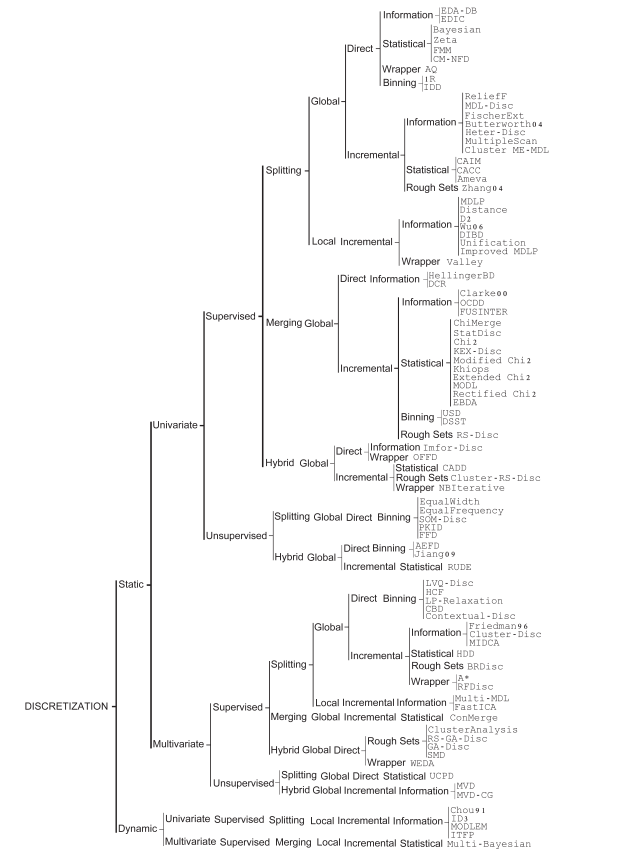
\includegraphics[height=1.36\linewidth]{obrazky/obrazok3}
	\caption{Taxonómia metód diskretizácie\cite{Garcia2013}}
	\label{fig:obrazok3}
\end{figure}




\begin{table}[p]
	\centering
	\begin{tabular} { |p{5cm}|p{10cm}| }
		\hline 
		\textbf{Kritérium diskretizácie} & \textbf{Príklady algoritmov} \\ 
		\hline 
		Statická & ChiMerge, MDLP, Chi2, RFDisc, UnDisc, CDisc, ME-MDL, ImformDisc, ImpMDLP \\ 
		\hline 
		Dynamická & ID3 a C45, MultiBayesian, MODLEM, ITFP \\ 
		\hline 
		Globálna  & EqualWidth a EqualFrequency, ChiMerge, Chi2, CAIM, RFDisc, UnDisc, ME-MDL, EBDA, ImforDisc \\ 
		\hline 
		Lokálna & MDLP, ID3 a C45, ImpMDLP \\ 
		\hline 
		Jednorozmerná & EqualWidth a EqualFrequency, MDLP, UnDisc, EBDA, ME-MDL, ImformDisc \\ 
		\hline 
		Mnohorozmerná & MVD, Multi-MDL, UCPD, MIDCA, WEDA, RFDisc, SMD, CBD \\ 
		\hline 
		Neriadená (bez učiteľa)  & EqualWidth a EqualFrequency, MVD, UnDisc, FFD \\ 
		\hline 
		Riadená (s učiteľom) & ChiMerge, MDLP, ID3 a C45, Chi2, WEDA, RFDisc, CDisc, EBDA, ME-MDL, ImforDisc, ImpMDLP \\ 
		\hline 
		Priama & UCPD, WEDA \\ 
		\hline 
		Inkremetálna (postupná) & ChiMerge, ID3 a CD45, Chi2, MVD, RFDisc, EBDA, ImpMDLP \\ 
		\hline 
		Neparametrická & MDLP, USD, CAIM \\ 
		\hline 
		Parametrická & ChiMerge, CADD \\ 
		\hline 
		Zlučovacia & ChiMerge, EBDA \\ 
		\hline 
		Rozdeľovacia & MDLP, RFDisc, CDisc, ME-MDL, ImpMDLP \\ 
		\hline 	Súčasná & HBD, IDD \\ 
		\hline 
		Hybridná  & CADD, WEDA, ImforDisc \\ 
		\hline 
		Informačných ukazovateľov & ID3 a C45, MDLP, DbEr, ME-MDL, ImforDisc, ImpMDLP, GINI \\ 
		\hline 
		Štatistických ukazovateľov & ChiMerge, Zeta, Chi2, EBDA, MODL \\ 
		\hline 
		Frekvenčných charakteristík & EqualWidth a EqualFrequency, UnDisc \\ 
		\hline 
		Presnosti klasifikácie & Valley, NBIterative, RFDisc \\ 
		\hline 
	\end{tabular} 
	\caption{Tabuľka príkladov algoritmov jednotlivých metód diskretizácie.}
	\label{table:1}
\end{table}
 



%%Vlastnosti niektorých známych algoritmov metód diskretizácie. 
%%\begin{itemize}
%%	\item EqualWidth a EqualFrequency - globálny, jednorozmerný, založený na frekvenčných charakteristikách\cite{Wong1987}. 
%%
%%\item
%%ChiMerge - statický, globálny, riadený, inkrementálny, parametrický, zlučovací, založený na štatistických ukazovateľov.
%%\cite{Keber1992} 
%%\item
%%ID3 a C45 - dynamický, lokálny, riadený, inkrementálny, založený na informačných ukazovateľov. 
%%\cite{Quinlan1993} 
%%
%%\item
%%MDLP - statický, jednorozmerný, riadený, neparametrický, rozdeľovací, založený na informačných ukazovateľov.
%%\cite{Fayyad1993} 
%%\item
%%Valley - založený na presnosti klasifikácie. 
%%\cite{Ventura1994} 
%%\item
%%NBIterative - založený na presnosti klasifikácie. 
%%\cite{Pazzani1995} 
%%
%%\item
%%CADD - parametrický, hybridný. 
%%\cite{Ching1995} 
%%\item
%%Chi2 - statický, globálny, riadený, inkrementálny, založený na štatistických ukazovateľov.
%%\cite{Liu1997} 
%%\item
%%
%%Zeta - založený na štatistických ukazovateľov. 
%%%Ho1997
%%\cite{Ho1997} 
%%\item
%%MultiBayesian - dynamický 
%%%Monti1998
%%\cite{Monti1998} 
%%\item
%%MODLEM - dynamický
%%%Grzymala2001
%%\cite{Grzymala2001} 
%%\item
%%MVD - mnohorozmerný, neriadný, inkrementálny. 
%%%Bay2001
%%\cite{Bay2001} 
%%\item
%%USD - neparametrický. 
%%%Giraldez2002
%%\cite{Giraldez2002} 
%%\item
%%CAIM - globálny, neparametrický. 
%%%Kurgan2004
%%\cite{Kurgan2004} 
%%\item
%%MIDCA - mnohorozmerný. 
%%%Chao2005
%%\cite{Chao2005} 
%%\item
%%UCPD - mnohorozmerný, priamy. 
%%%Mehta2005
%%\cite{Mehta2005} 
%%\item
%%Multi-MDLP - mnohorozmerný.
%%%Ferrandiz2005
%%\cite{Ferrandiz2005} 
%%\item
%%MODL - založený na štatistických ukazovateľov. 
%%%Boulle2006
%%\cite{Boulle2006} 
%%\item
%%ITFP - dynamický
%%%Au2006
%%\cite{Au2006} 
%%\item
%%HBD - súčasné zlučovanie/rozdeľovanie niektoľkých intervalov. 
%%%Lee2007
%%\cite{Lee2007} 
%%\item
%%WEDA - mnohorozmerný, riadený, priamy, hybridný. 
%%%Flores2007
%%\cite{Flores2007} 
%%\item
%%IDD - súčasné zlučovanie/rozdeľovanie niektoľkých intervalov. 
%%%Ruiz2008
%%\cite{Ruiz2008} 
%%\item
%%DbEr - založený na informačných ukazovateľov. 
%%%Hu2008
%%\cite{Hu2008} 
%%\item
%%RFDisc - statický, globálny, mnohorozmerný, riadený, inkrementálny, rozdeľovací, založený na presnosti klasifikácie.
%%%Berrado2009
%%\cite{Berrado2009} 
%%\item
%%UnDisc - statický, globálny, jednorozmerný, neriadný, založený na frekvenčných charakteristikách.
%%%Jiang2009
%%\cite{Jiang2009} 
%%\item
%%GINI 
%%%Jin2009 - založený na pojmoch teórie informácie. 
%%\cite{Jin2009} 
%%\item
%%FFD - neriadný. 
%%%Yang2009a
%%\cite{Yang2009a} 
%%\item
%%SMD - mnohorozmerný. 
%%%Jiang2009
%%\cite{Jiang2009} 
%%\item
%%CDisc - statický, riadený, rozdeľovací, 
%%%Nemmiche2010
%%\cite{Nemmiche2010} 
%%\item
%%ImforDisc - statický, globálny, jednorozmerný,  riadený, hybridný, založený na informačných ukazovateľov.
%%%Zhu2010
%%\cite{Zhu2010} 
%%\item
%%ImpMDLP - statický, lokálny, riadený, inkrementálny, rozdeľovací, založený na informačných ukazovateľov. 
%%%Li2010a
%%\cite{Li2010a} 
%%\item
%%ME-MDL - statický, globálny, jednorozmerný, riadený, rozdeľovací, založený na informačných ukazovateľov.
%%%Gupta2010
%%\cite{Gupta2010} 
%%
%%\item
%%EBDA - globálny, jednorozmerný, riadený, inkrementálny, zlučovací, založený na štatistických ukazovateľov. 
%%%Sang2010
%%\cite{Sang2010} 
%%\item
%%CBD - mnohorozmerný. 
%%%Garcia2010
%%\cite{Garcia2010} 
%%
%%\end{itemize}


















\section{Meranie Entropie}
Entropia je meraná množstvom neistoty výsledku náhodného experimentu, alebo equivalene, meraním informácií, keď sa pozoruje výsledok. Tento koncept bol zadefinovaný rôznymi spôsobmi \cite{kosko25, renyi30} a zovšeobecnený v rozličných aplikovaných oblastiach, ako napríklad teória komunikácie, matematiky, štatistickej termodynamike a ekonómii \cite{belahut31, cover33}. Z pomedzi týchto rozličných definícií, Shannon prispel k najširšej a naj fundamentálnejšej definícii entropie v informačnej teórii. 
% * <eruner@azet.sk> 2017-04-17T19:15:05.601Z:
% 
% to slovo "equivalene" tam má byť alebo to chce slovenskú verziu toho slova?
% 
% ^.

\subsection*{Shannonova Entropia}
Za entropiu možno považovať meranie neistoty náhodnej premennej $X$.
\begin{defn} 
	Nech $X$ je náhodná spočítateľná premenná s konečnou \textit{N}-znakovou abecedou danou $ \left\{ x_0, x_1, \dots, x_{N-1} \right\}$.
	Ak výsledok $x_j$ sa vyskytuje s pravdepodobnosťou \textit{p($x_j)$}, tak potom množstvo informácie spojené so známym výskytom výstupu $x_j$ je definované ako:
	$$ I(x_j)=-\log_z p(x_j). $$
\end{defn}
To znamená, že pre diskrétne zdroje, informácie získané výberom symbolu $x_j$ sú $\lceil \log_zp(x_j)  \rceil$ bitové. V priemere, symbol $x_j$ bude vybratý $n*p(x_j)$-krát z celkového počtu $N$ výberov, takže priemerné množstvo informácie získanej zo zdrojových výsledkov je:

$$
-n.p(x_0)\log_2p(x_0) - n.p(x_1)\log_2p(x_1) - \ldots 
-n.p(x_{N-1})\log_2p(x_{N-1}).
$$

Podelením výrazu číslom $n$ sa získa priemerné množstvo informácie na symbol výskytu zdroja. To je známe ako priemerná informácia, neistota, alebo entropia definovaná nasledovne.

\begin{defn}  Entropia $H(X)$ náhodnej diskrétnej premennej $X$ je definovaná ako 
	$$H\left(x\right)=-\sum\limits_{j=0}^{N-1}p\left(x_j\right)\log_2p\left(x_j\right) $$
	
	alebo
	
	$$H\left(x\right)=-\sum\limits_{j=0}^{N-1}p_j
	\log_2p_j$$.
\end{defn}
Entropia je funkcia distribúcie $X$. Nezáleží na skutočných hodnotách náhodnej premennej $X$, ale iba na pravdepodobnostiach. Preto entropiu možno zapísať ako $H(p)$.
\subsection*{Luca-Termini Axiómy}
Kosko \cite{kosko25} navrhuje, aby meranie dobre definovanej fuzzy entropie musí spĺňať štyri Luca-Termini axiómy. Patria medzi ne nasledujúce:
\begin{itemize}
	\item $E(A)=0 \iff A\in 2^X $, kde 
	$A$ nie je fuzzy množina a $2^X$ je množina všetkých podmnožín množiny 
	$A$. 
	
	\item
	$E(\tilde{A}) =1 \iff m_{{A}}(x_i) =0.5$ pre všetky $i$, kde $m_{\tilde{A}}(x_i)$
	znamená stupeň príslušnosti 
	$x_i$ 
	v fuzzy množine $\tilde{A}$. \item $E(\tilde{A}) \leq E(\tilde{B}) $,  ak 
	$\tilde{A}$ je menej fuzzy než $\tilde{B}$, napr. ak $m_{\tilde{A}}(x) \leq m_{\tilde{B}} (x)$,  keď 
	$m_B(x) \leq 0.5$ a $m_{\tilde{A}}(x) \geq m_{\tilde{B}}(x)$, 
	keď $m_B(x) \geq 0.5$, kde $\tilde{A}$ aj $\tilde{B}$ sú fuzzy množiny. 
	\item 
	$E(A)=E(A^C)$.
\end{itemize} 


\subsection*{Fuzzy entropia na intervale pre každú vlastnosť v rozmere}


\begin{defn}Definícia fuzzy entropie na základe Shannonovej entropie. 
\begin{itemize}
	\item[1)] Nech $X={r_1,r_2,\ldots,r_n}$ je univerzálna množina prvkov $r_i$ rozptýlená v vzorkovom priestore, kde   $i=1,2, \ldots, n$. 
	
	\item[2)]
	Nech $\tilde{A}$  je fuzzy množina definovaná na intervale vzorkového priestoru, ktorý obsahuje $k$ elementov ($k<n$). Na mapovanie stupňa príslušnosti elementu $r_i$
	s fuzzy množinou $\tilde{A}$  sa označuje ako 
	$\mu_{\tilde{A}}(r_i)$. 
	
	\item[3)]
	Nech $C_1, C_2, \ldots,C_m$  reprezentujú $m$  tried, v ktorých je rozdelených $n$ elementov. 
	
	\item[4)]
	Nech $S_{C_j}(r_n)$  je množina elementov triedy  $j$  na univerzálnej množine $X$.
	Je to podmnožina univerzálnej množiny $X$. 
	
	\item[5)]
	Stupeň príslušnosti elementov fuzzy množiny $\tilde{A}$
	triedy $j$ na intervale, kde $j=1,2,\ldots,m$
	je definovaný ako: 
	\begin{equation}
	{D_j} = \frac{
		\sum\limits_{r\in S_{C_j}(r_n)}
		\mu_{\tilde{A}}(r)
	}{
		\sum\limits_{r \in X}
		\mu_{\tilde{A}}
		\left(r\right)
	}. 
	\end{equation}
	
	\item[6)]
	Fuzzy Entropia $FEC_j(\tilde{A})$ elementov triedy $j$
	na intervale je definovaná ako: 
	\begin{equation}\label{eq:eq6}
	FEC_j(\tilde{A}) = -D_j \log_2D_j.
	\end{equation}
	\item[7)]
	Fuzzy Entropia $FE(\tilde{A})$ na univerzálnej množine $X$
	pre elementy v intervale je definovaná ako: 
	$$
	FE(\tilde{A}) = \sum\limits_{j=1}^m FE_{C_j}(\tilde{A}). 
	$$
	
\end{itemize}
\end{defn}


Vo výraze \ref{eq:eq6} je fuzzy entropia $FEC_j(\tilde{A})$  ako nepravdepodobnostná entropia. Preto môžme zadefinovať nový pojem stupeň príslušnosti pre $D_j$. Základná vlastnosť navrhnutej fuzzy entropie je podobná ako Shannonova entropia a spĺňa štyri Luca-Termini axiómy, ale ich spôsob merania informácie je rôzny. Pravdepodobnosť $p_j$ Shannonovej entropie je meraná cez výskyt elementov. Oproti tomu, stupeň príslušnosti $D_j$ v fuzzy entropii je merané príslušenstvom hodnôt vyskytujúcich sa elementov. Okrem toho, fuzzy entropia rozhodovacích oblastiach môže byť získaná cez súčet fuzzy entropie jednotlivých intervalov v každej dimenzii vlastností. \cite{lee2001}

Takto zadefinovaná fuzzy entropia je lepšie schopná rozlíšiť skutočné rozloženie vzorov. Použitím funkcie príslušnosti pre meranie stupňa príslušnosti, hodnota entropie obsahuje nie len počet, ale aj berie do úvahy rozloženie vzorov.  \cite{lee2001}




























